\section{\tc Implementation Details}
\label{sec:impl}

\subsection{TC Contract}

To implement the TC Contract we implemented the version of \tcont including fees and cancellation as described in Section~\ethan{ref}.
The contract is implemented in Solidity, a high-level language with JavaScript-like syntax which compiles to Ethereum Virtual Machine bytecode---the language that can be executed as a contract on the blockchain.

In order to handle the most general type of requests---including encrypted parameters---the \tcont implementation requires two parameter fields.
The first specifies what type of request is being made (e.g. stock price or flight status).
The second is a byte array of user-specified size.
This byte array will be parsed and interpreted inside the enclave when it fulfills the request, but is treated as an opaque byte array by \tcont.

As we discuss in Section~\ethan{ref authenticity}, TC must pass the entire byte array back to {\bf Deliver} to ensure that the request has not been modified.
Unfortunately, this verification (as well as Ethereum's cost on each byte in a transaction) means the size of this byte array greatly affects the cost of calling the {\bf Deliver} entry point.
In fact, when the byte array contains 400 bytes of data, this extra cost outweighs all other costs of {\bf Deliver} combined (not including \dgcallback).
In order to achieve our desired guarantees of cost while not demanding excessive fees for requests which supply only a few bytes of data,
our implementation scales the minimum fee with the length of the user provided byte array.



\subsection{TC Server}
% programming model
% ecall and ocall

\subsubsection{Overview of SGX-enabled applications}

Using the recently released Intel SGX SDK~\cite{sgxsdk}, we implmented the \tc
Server as an SGX-enabled application in C++. The programming model employed by
the SDK is that the major body of an SGX-enabled application remains an
ordinary user-space application, while an relatively small piece of security-sensitive code
is teased out and runs in an isolated environment, namely in an SGX enclave.

The enclave part of an SGX-enabled application can be
viewed as a shared library exposing APIs, referred to as \emph{ecalls} by~\cite{sgxsdk},
to be invoked by the untrusted application. However, unlike a share library,  
once ecalls are invoked, the control is transferred to the 
enclave code until it finishes or some special event happens~\cite{sgxmanual}.
As we assume SGX provides a perfect isolation, the untrusted application can not
observe or alter the execution of ecalls.

In addition, the SGX SDK implements a mechanism called \emph{ocall} with which enclave
programs can invoke functions defined outside of the enclave. In essence,
calling an ocall causes the enclave program first to exit the enclave. Once the
ocall is fulfilled, execution is transferred back to the calling enclave. 
Although it is permissible to make arbitrary ocalls, special caution must be 
as ocalls are fulfilled in the untrusted world.
The ocall interface between \encname and \medname is carefully designed such that the 
the \medname can not subvert the security of \tc.

In the context of TC Server, the enclave part implements Figure. \fan{ref to
prog}, which encompasses the implementation of a TLS layer, a partial HTTP
layer, a set of algorithms that extract information from web pages, and a
request handler that can parse and generate Ethereum transactions and sign it
properly with \skTC.  The untrusted part of TC Server implements Figure \fan{ref
to prog}, which roughly encompasses of two parts: (1) an access point to various
OS services, (2) an interface with Ethereum blockchain and (3) an interface with
clients. Figure \ref{fig:tcserver_impl} summarizes these components and their
interaction.

\begin{figure}[h]
    \centering
    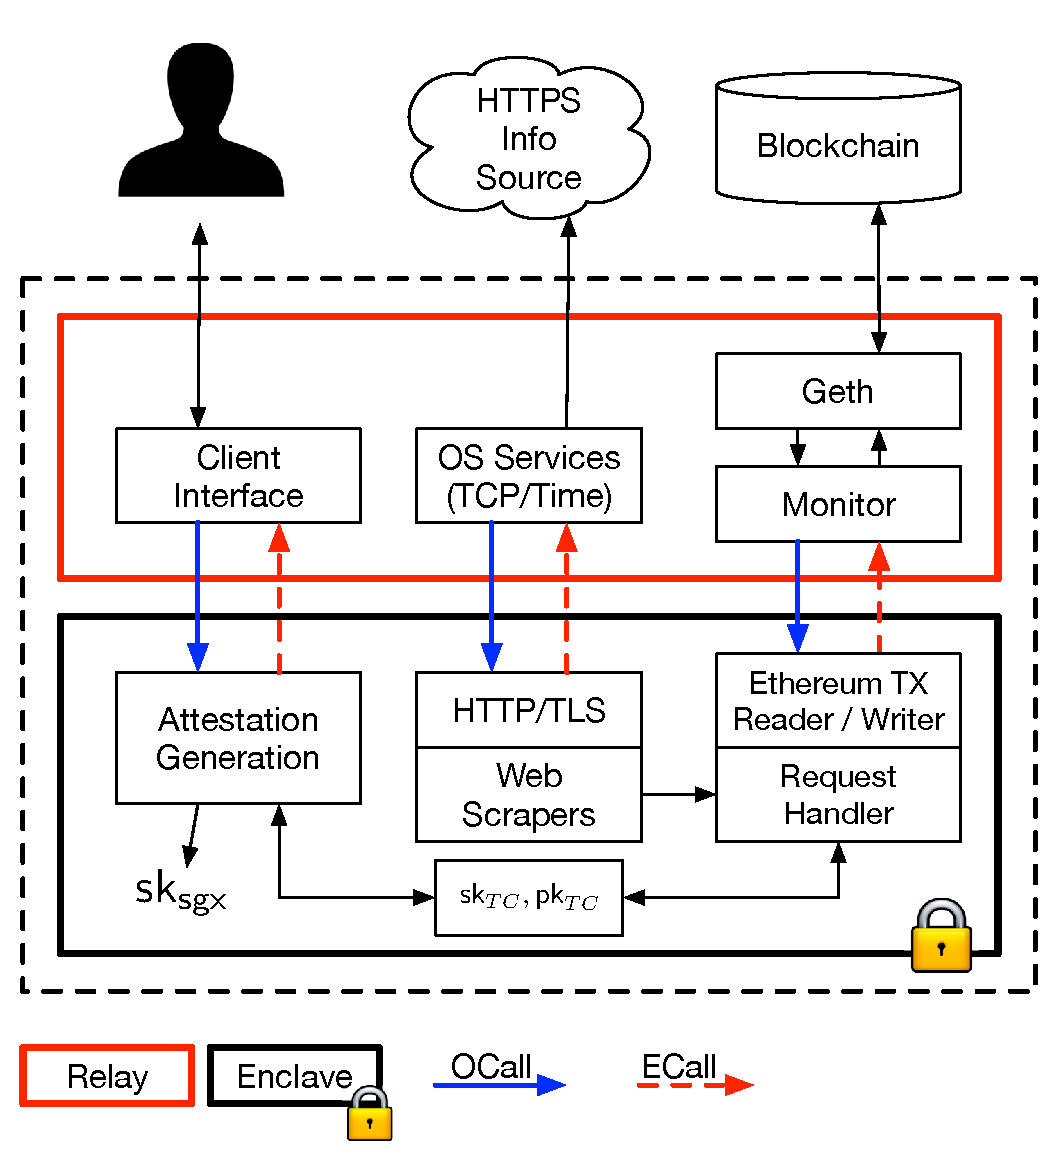
\includegraphics[width=0.4\textwidth]{figures/impl}
    \caption{Detailed Architecture of TC Server}
    \label{fig:tcserver_impl}
\end{figure}

\subsubsection{The \medname}

\paragraph{Attestation Server.} As described in Section \ref{sec:architecture},
a client starts using \tc by requesting and verifying an attestation.  The
Attestation Server (AttServer) is the interface for doing this.  The AttServer
listens for requests and calls into the Attestation Generation logic in the
enclave (by making an ecall) to get an attestation, along with an Unix timestamp
signed by \pkTC, and forward both to the requesting client.  The EPID group
signature can verified by accessing Intel Attestation Service (IAS)~\cite{}. 

\paragraph{OS Services.} The \encname relies on \medname for networking and
time provided by the OS. We implemented wrapper functions for these OS services 
that can be invoked by the \encname as ocalls.

\paragraph{Blockchain Interface.} The \medname is responsible to watch the
blockchain for incoming requests and insert transactions to the blockchain to
deliver datagrams. To interact with the Ethereum blockchain, we incorporated an
official Ethereum client (geth~\cite{geth} in particular) into the \medname.
Geth client can be configured to setup a JSON RPC server through which the
Monitor can communicate with the blockchain indirectly by sending RPC calls to
geth. For example, to insert a signed transaction, the Monitor can simply call
\texttt{eth\_sendRawTransaction} with the bytes array of the serialized
transaction, and geth do the rest of the work. Looping an Ethereum
client into \medname saves us the cost of reinventing the wheel. 
Note that the signing of transactions is done within the enclave, as the key
\pkTC only accessible to the enclave program.

\subsubsection{The \encname}

\paragraph{HTTPS in the \encname.} 
The \encname needs the TLS layer to talk with remote HTTPS web servers.  We
ported a TLS library (mbedTLS) into the SGX environment so it can be used within
the enclave.  To verify the certificates presented by remote servers, a
collection of trusted root CAs are manually selected \xxx[Fan]{what's the best
practice? Maybe we can choose the same root CAs as Chrome or Firefox?} and their
certificates are hardcoded in the enclave program. A certificate is verified
only if it is finally issued by one of the trusted root CA.

\paragraph{Web Scrapers.} Extracting useful information from a given website is
implemented in a ad-hoc manner. For the purpose of demonstration, we implemented
three web scrapers as examples. \xxx[Fan]{Elaborate}.

\paragraph{Request Handler} Request handler has two jobs: 1) to parse the
request which is serialized in the format specified by Ethereum ABI, decrypt it if encrypted under
\pkTC, and dispatch it to the right scraper; 2) to generate a Ethereum
transaction, sign it with \pkTC and serialize it properly so that it can be
inserted to the blockchain. In essence, we implemented the Ethereum ABI and RLP which
specifies the serialization of arguments and transactions respectively.
In addition, the signature algorithm used in signing Ethereum transactions is
ECDSA on the curve Secp256k1. SHA3 is used to generate message digests.

\paragraph{Attestation Generation} The same with Attestation Server.\xxx[Fan]{Elaborate.}
\paragraph{Key Management} \xxx[Fan]{TBD.}


